\chapter{The Argumentation on the Social Web Ontology}
\label{aswo}
In the preliminary investigation, the capability of existing frameworks and their use in capturing and modelling argumentation and social communities was examined and evaluated \citep{Blount2014}. It became apparent that the AIF, while a powerful tool for modelling (dialectic) argument, lacked the ability to capture the eristic aspects of social argumentation. While some logical fallacies, such as the \textit{ad hominem} attack can be suitably modelled within the AIF, the rhetorical force of ``simple'' abuse is difficult to capture. 

However, there is reason to suggest that while such abuse (for example) may not be valuable to the argument$_2$ itself, that does not mean it is not valuable to model such outbursts. A heckler in a debate, for example, may not have any well-reasoned argument$_1$ to hand and resort to throwing vulgarities, but by simply disrupting the proceedings they are voicing their dissent at the positions offered. This is reason enough not to discard the contribution; however, it can also act to catalyse further argumentation on the subject between the main participants. Likewise, a participant in a debate may, instead of putting forth their own argument or attacking their opponent's, make some sort of joke to endear themselves to the audience. While the AIF can model the locution, the rhetorical force behind it goes uncaptured.

In addition, there are other socio-rhetorical tactics that are often employed on social media. These include spamming (posting large volumes of a repetitive nature) to drown out other posters, deliberate deviation from the topic at hand, bringing up non-sequiturs in an attempt to derail the argument and ``meta-argumentation'' -- criticising the way in which an opponent argues, but not the argument itself (e.g. if a user claims another is breaking the rules of the forum, or of not arguing in good faith). There are also the non-textual features of social media to consider; that is, the feature of posts other than their content. For example, the number of ``Likes'' or ``Favourites'' a post has, demonstrates popular (or audience) support for this opinion or position. 


\section{Initial Proposals}
\label{aswo:augmentations}

\newcommand{\scaleProps}{0.7}

\TODO{Discuss different proposals, pros and cons, why settled on final choice}

%These results formed the basis for the work presented in the Workshop on Computational Models of Natural Argument, in which a number of suggestions on how these ontologies could be adapted to model the socio-rhetorical aspects of argumentation were proposed.

The principal focus here is the inclusion of rhetorical support and attack. While these features are only one aspect of rhetorical argument, they feature heavily in eristic dialogue (particularly rhetorical attacks), showcase both the positive and negative aspects of rhetorical argument and are important due to the impact they can have within discussions on the social web and the culture surrounding it \citep{Blount2015}.

Rhetorical support is often relatively benign. It can be used to show solidarity with other members of the dialogue, to incorporate oneself into a social group, or to encourage . Consider the extracts \textit{``bro fist bump''}, a short declaration of support for another user, and \textit{``I commend you for admitting that debt \& deficits are important...If only more [people] felt the way you do''}, which disagrees with the overall stance presented by their opponent, but commends them for conceding some common ground, in attempt to further dialectic argument.

Conversely, rhetorical attacks are often extremely hostile. They differ from logical attacks by attacking the person behind the argument rather than the argument itself (this is not to be confused with an \textit{ad hominem} argument which attacks a person's argument by calling their character or credentials into question -- these are logical, even though they are fallacious). Rhetorical attacks often contain extremely vulgar language.
%: consider the extracts \textit{``Some of you fucks need a good ass whipping''} and \textit{``Fuck off cunt''}. \TODO{Do I need to censor this?}
The purpose of these statements can be interpreted in a number of ways, from showing the audience how impassioned and emotive the rhetor is on the subject, to cathartically blowing off steam, to intentionally silencing dissenting voices with threats.

Figure \ref{figure:cmna:abuse1} shows the simplest approach, similar to the current way the AIF models the use of \textit{ad hominem} attacks, by linking the attack to the opponent's argument$_1$ with a CA-node. However, this is insufficient for the majority of abusive attacks; while \textit{ad hominem} tactics attack an opponent's argument$_1$ by claiming they are not qualified, or otherwise unfit, to make such an argument$_1$, abuse often does not attack their position at all, but seeks to undermine them emotionally in front of their peers.

This mapping can be modelled by linking the content of the locution to the targeted user's account as shown in Figure \ref{figure:cmna:abuse2}. However, a UserAccount can be involved in any number of topics, and be attacked for any number of reasons. Furthermore, a person can choose to present themselves as a dramatically different person (having different credentials, skills, opinions or even race, religion or gender) when they are on the web as opposed to off. They may even choose to represent themselves differently between individual threads and discussions. To this end, another type of node is needed to represent the abstract notion of the ``persona'' a user presents.

This is illustrated by Figure \ref{figure:cmna:abuse3}. Introducing the idea of personas allows each UserAccount to present a different view of themselves (that can be supported or attacked accordingly) when engaging in multiple discussions or topics.

Figure \ref{figure:cmna:abuse4} \TODO{Shows persona nodes}

Here, the key additions is the Persona node -- this represents ``character'' that they assume during the discussion. A person may argue in a different fashion in a debate about music than they would about technical expertise, for example. This allows one UserAccount to have many Personas where necessary. The inverse, linking one Persona to multiple UserAccounts, is also possible, and could represent a participant attempting to artificially solidify their position by creating multiple accounts.


\begin{figure}
\centering
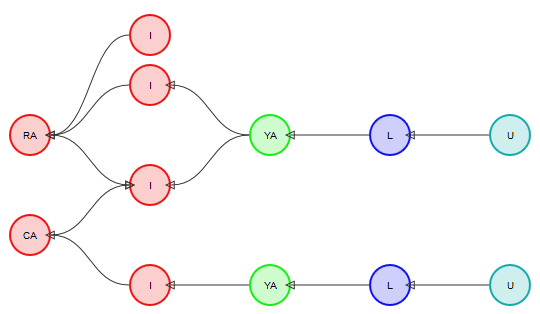
\includegraphics[scale=\scaleProps]{./figures/cmna_proposals/abuse1.png}
\caption{Proposal for representing abusive attacks as solely within the argument$_1$ structure}
\label{figure:cmna:abuse1}
\end{figure}

\begin{figure}
\centering
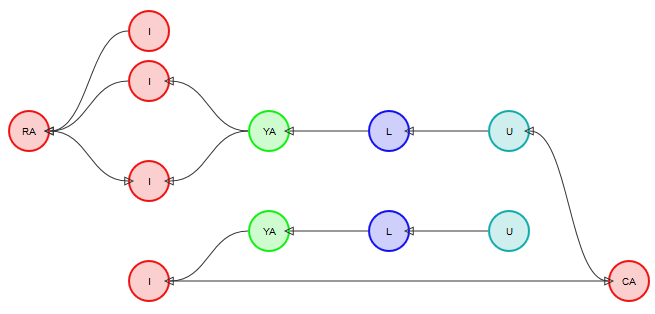
\includegraphics[scale=\scaleProps]{./figures/cmna_proposals/abuse2.png}
\caption{Proposal for representing abusive attacks as connected with the social aspect of the argument$_2$, attacking the author directly}
\label{figure:cmna:abuse2}
\end{figure}

\begin{figure}
\centering
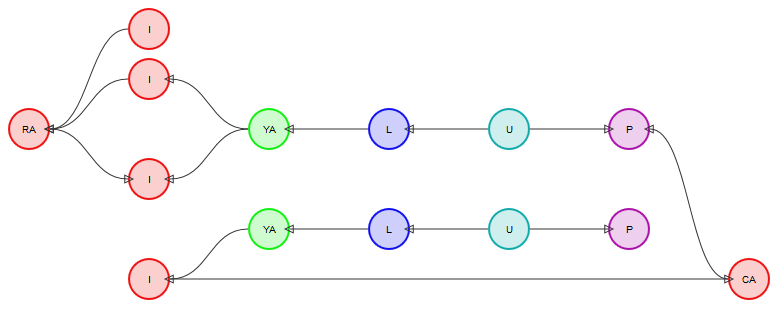
\includegraphics[scale=\scaleProps]{./figures/cmna_proposals/abuse3.png}
\caption{Proposal for representing abusive attacks, extending that shown in Figure \ref{figure:cmna:abuse2} with the addition of Persona nodes}
\label{figure:cmna:abuse3}
\end{figure}

\begin{figure}
\centering
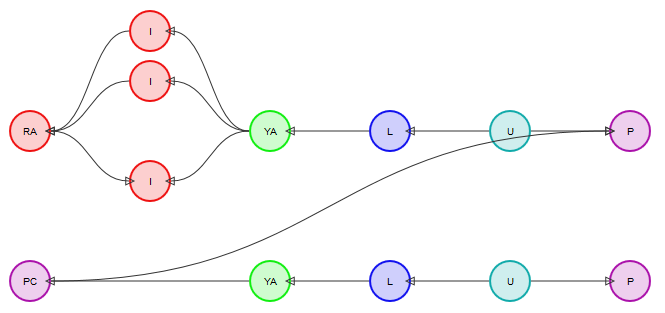
\includegraphics[scale=0.5]{./figures/graphs/aswo-personal-conflict.png}
\caption{Proposal for representing abusive attacks, extending that shown in Figure \ref{figure:cmna:abuse3} with the addition of Personal Conflict node}
\label{figure:cmna:abuse4}
\end{figure}

%%%%%%%%%%%%%%%%%%%%%%%%%%%%%%%%%%%%%%%%%%%%%%%%%%%%%%%%%%%%%%%%%%%%%%%%%%%%%%%%%%%%

\TODO{while out of scope for this body of work, the topic of modelling social systems was also considered} \citep{Blount2014}. These proposals included suggestions for modelling social web specific features, such as the use of reputation systems (e.g. Likes or up/down-votes). Reputation systems make up a key aspect of non-verbal argumentation on the social web, allowing users to show agreement or disagreement to a position, sometimes anonymously, without the need to articulate their own position.

Figure \ref{figure:cmna:likes1} shows one such approach; namely, modelling each vote as a separate Locution, linking to an I-node that either (logically) supports or attacks the voted-on post.

Alternatively, Figure \ref{figure:cmna:likes2} shows an approach which aggregates this information into a single Reputation node. This has the advantage of keeping to social information distinct from the logical graph structure, but the disadvantage of omitting how much each UserAccount contributed to the reputation.

The ASWO does model these  reputation systems; however, for simplicity, they are not modelled as nodes in the graph structure, but are included as literal values attached to the relevant Locution. 


\begin{figure}
\centering
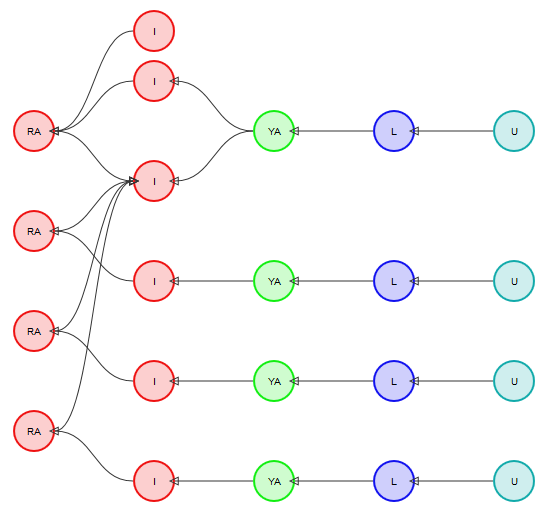
\includegraphics[scale=\scaleProps]{./figures/cmna_proposals/likes2.png}
\caption{Proposal for representing reputation systems by modelling up- and down-votes as individual Locutions}
\label{figure:cmna:likes1}
\end{figure}

\begin{figure}
\centering
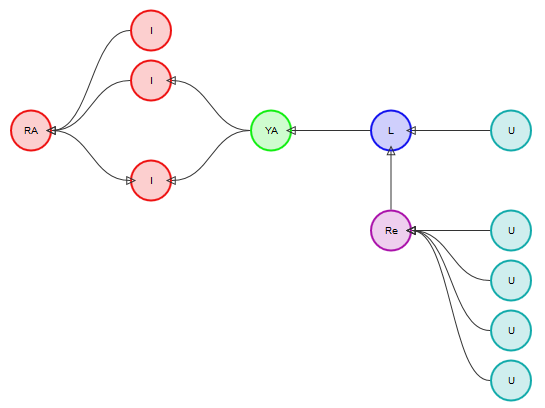
\includegraphics[scale=\scaleProps]{./figures/cmna_proposals/likes1.png}
\caption{Proposal for representing reputation systems with the introduction of a Reputation node}
\label{figure:cmna:likes2}
\end{figure}

In addition, because the SIOC ontology also accounts for replies to and from a post, the use of AIF TA-nodes has also been refined in relation to the social web. They now no longer need to be used whenever an L-node directly responds to another; instead they can be used solely to refer to ``transitions'' in the argument. These transitions are used when a Locution contributes to the argument$_2$ without providing any information, but instead helps move the discussion to the ``next stage'', usually by asking questions or prompting further debate. Note that these transitions don't necessarily move the discussion forwards, but can also be used to take the argument$_2$ around in circles by asking questions in bad faith (or \textit{sealioning}).

%%%%%%%%%%%%%%%%%%%%%%%%%%%%%%%%%%%%%%%%%%%%%%%%%%%%%%%%%%%%%%%%%%%%%%%%%%%%%%%%%%%%%%%%%%%%

\TODO{TIE THESE BITS TOGETHER}

%Based on the observations made in Section \ref{investigation:results} and the proposals discussed in Section \ref{investigation:proposals}, the principal features from the AIF and SIOC ontologies are combined alongside means to model rhetorical tactics in the Argumentation on the Social Web Ontology (ASWO).



%The notion of rhetorical support and attack is modelled by introducing three new types of nodes to the ontology. Firstly, as described in Section \ref{investigation:proposals}, it is not enough to use a UserAccount to represent a person during an argument$_2$. Instead, the Persona node represents a user's character and authority on a given subject, or rather the character and authority they present themselves to have online, and is bound to one or more UserAccounts. Two more node types are introduced to differentiate these types of rhetorical interaction from logical supports or attacks. PersonalConflict (PC-nodes) nodes link from a YA-node to a Persona node to denote this type of personal support and, likewise, PersonalSupport (PS-nodes) nodes follow the same structure to denote support of a person's intentions and character. These are broad, umbrella definitions that serve to catalogue all discovered variants of personal support and attack; they could of course be refined to differentiate between different subcategories of support, such as simple agreement, or self-support (through humour, etc.), or attack such as threats, insults, or provocations. A simple example of this is shown in Figure \ref{figure:graphs:aswo-personal-conflict}, \TODO{MOVED FIGURE} which shows the same argument visualised in Figure \ref{figure:graphs:aifplus} (with the addition of User and Persona nodes) being rhetorically attacked by another user.


\section{Investigation}
\label{aswo:investigation}
The ASWO, and the augmentations made to the AIF and SIOC ontologies, were trialled in an investigation to study the application of logical versus rhetorical techniques in eristic dialogue on the social web. As before, this investigation focused on three different areas of the social web, but used a much larger sample size than previously: in total, two hundred and seventy posts were collected and annotated. These were used to analyse the proportion of rhetorical contributions throughout the argument$_2$, analyse the relation between logical and rhetorical arguments$_1$ used, and compare the features of the annotation structure with the content of each post.


\subsection{Methodology}

\subsubsection{Data Collection}
During the course of this work, the Google YouTube API v2.0 was deprecated before the API v3.0 fully supported the retrieval of explicit replies to comments. Due to the importance of the ability to capture replies, the decision was made to use an alternative medium in this case study. To this end, YouTube was replaced with the social news and networking site Reddit. Reddit has a variety of topic-specific boards or ``subreddits'' that allow users to post to a collaborative pool of information; posts can then be up-voted or down-voted to show interest and/or accuracy.

Obama's official account on Reddit was inactive over the period of the shutdown; however, another user (unaffiliated in any official capacity with Obama) posted a link to Obama's official website (managed by Organizing for Action) to Reddit's politics subreddit\footnote{http://reddit.com/r/politics/1oij25} on 15th October 2013 (the same date as the official posts to Twitter and Facebook). The post reads \textit{``Tea Party Republicans in the House of Representatives have already shut down the government because they couldn't derail Obamacare. Now they're threatening to cause an economic shutdown''}. This thread was used alongside the previously acquired threads from Twitter and Facebook described in Section \ref{investigation:methodology:datacollection}. Each UserAccount involved in the three threads was automatically designated a single Persona, as only one topic was monitored. This could be expanded if the same UserAccount took part in multiple threads on multiple topics, for example.


\begin{table}
\centering
\caption{Metrics of discussions sampled from Twitter, Facebook and Reddit}
\label{table:samples}
\begin{tabular}{| l | c | c | c | c |}
\hline
\textbf{Metric} & \textbf{Twitter} & \textbf{Facebook} & \textbf{Reddit} & \textbf{Total}\\
\hline
Posts & 90 & 90 & 90 & 270\\
\hline
Direct replies & 77 & 0 & 67 & 144\\
\hline
Number of users & 26 & 85 & 43 & 154\\
\hline
Average posts per user & 3.5 & 1.1 & 2.1 & 1.8\\
\hline
Average words per post & 15.83 & 41.36 & 42.34 & 33.18\\
\hline
Average characters per post & 96.51 & 265.27 & 243.31 & 201.70\\
\hline
Time between first and last posts & 0d 6h 53m 40s & 3d 4h 51m 27s & 3d 0h 50m 12s & n/a\\
\hline
Average time between posts & 04m 39s & 51m 49s & 49m 06s & 35m 11s\\
\hline

\end{tabular}
\end{table}

As with the preliminary work, forest fire sampling of the graphs was undertaken to provide a representative sample of the arguments that was feasible to annotate manually. For this investigation a larger sample size of ninety posts was used from within each discussion. Table \ref{table:samples} shows an overview of the sample structures and some key characteristics of each thread.


\subsubsection{Annotation}
\label{aswo:investigation:annotations}
With the changes to the ontologies in use (such as the decision regarding TA-nodes discussed in Section \ref{aswo:augmentations}), and a larger amount of data needing to be annotated, the annotation method itself needed to be properly formalised to solidify reproducibility and minimise subjectiveness. Posts are annotated according to the scheme below.

Each post is considered to contain zero or more separate arguments$_1$. A YA-node is created for each argument$_1$ made in a single post, and links the L-node to each I-node in the argument$_1$. Repeated information does not create a new I-node; instead the YA-node links to the I-node already present. All participants are assumed to have some implicit knowledge about the world in general and the topic at hand. This is to avoid the inclusions of trivial I-nodes that state information such as \textit{``Barack Obama is president of the United States''}, or even \textit{``Barack Obama is a human being''}. Any information explicitly contained in a post that is deemed to be not in this set and relevant to the discussion at hand was included as an I-node. Information that meets one (or more) of the following criteria is not considered relevant:

\begin{itemize}
	\item Off topic: posts that do not relate to the topic being discussed are not considered relevant. Example: \textit{``Ataturk did revolution ! building moderate muslim network is oxymoron which has been destroy secular , democratic, rule of law in Turkey.''}
	\item Conversational: similar to off-topic posts, those that are conversational in nature are not annotated as information-containing. Example: \textit{``I thank you, have a good night!''}
	\item Meta-argumentation: while argumentation about how to argue ``properly'' is an interesting construct in itself, and an important aspect of rhetorical and eristic argumentation, but was out of scope for this particular study. Example: \textit{``Down voting = disagree Upvoting = agree''} \textit{``The rules say explicitly not to do that.....''}
\end{itemize}

A TA-node is created to link two Locutions whenever a transition is present in the argument$_2$ -- a step that contributes to the overall structure without providing any information (new or repeated). This is most often in the form of an interrogative (for example, asking for further information or evidence for claims). Support and attack between different I-nodes is denoted as described above: logical support through the use of RA-nodes, attack through the use of CA-nodes and preference with PA-nodes, while rhetorical support and attack utilises the new PS- and PC-nodes.

Some nodes in the graph may not be complete as a result of the nature of sampling the graph. For example, it may be possible to detect that a user attacks another user's persona, but not exactly which user they are attacking. Table \ref{table:aifnodes} shows an overview of the number of AIF and ASWO nodes added during the annotation process.

\begin{table}
\centering
\caption{Summary of AIF and ASWO nodes found in annotated discussions collected from Twitter, Facebook and Reddit}
\label{table:aifnodes}
\begin{tabular}{| l | c | c | c | c |}
\hline
\textbf{Metric} & \textbf{Twitter} & \textbf{Facebook} & \textbf{Reddit} & \textbf{Total}\\
\hline
L-nodes & 90 & 90 & 90 & 270\\
\hline
TA-nodes & 52 & 9 & 15 & 76\\
\hline
YA-nodes & 58 & 74 & 70 & 202\\
\hline
I-nodes & 56 & 98 & 86 & 240\\
\hline
RA-nodes & 13 & 20 & 24 & 57\\
\hline
CA-nodes & 18 & 1 & 34 & 53\\
\hline
PA-nodes & 4 & 4 & 2 & 10\\
\hline
PS-nodes & 2 & 2 & 3 & 7\\
\hline
PC-nodes & 26 & 6 & 12 & 44\\
\hline
L- to I-node Ratio & 45:28 & 45:49 & 45:43 & 9:8\\
\hline
\end{tabular}
\end{table}


\subsection{Results and Analysis}
\label{aswo:results}

\newcommand{\scaleResults}{0.4}

\subsubsection{Argumentation Tactics Over Time}
Firstly, the way in which the argumentation structure changes and grows over time is presented, in both a logical and rhetorical capacity, by graphing how the number of logical support and attack nodes (i.e. RA- and CA-nodes) and rhetorical support and attack nodes (i.e. PS- and PC-nodes) changes with each post contributed to the argument$_2$. Logical contributions are displayed above the x-axis, and rhetorical contributions below. It must be emphasised that values below the x-axis of each graph should \textit{not} be considered as inherently negative, hostile or anti-social; they simply differentiate between the two types of content.

Figures \ref{figure:rhetorictime:Facebook} and \ref{figure:rhetorictime:reddit} show that use of rhetorical tactics in the Facebook and Reddit case studies rise slowly compared to the use of logical tactics. However, Figure \ref{figure:rhetorictime:Twitter} shows that in the Twitter case study, the rhetorical contributions rise in parallel to the logical contributions.

In both samples from Twitter and Reddit, the distribution of logical supports and attacks also remain approximately equal. Due to the tendency of RA-nodes to be used for logical support within an argument$_1$, and the tendency of CA-nodes to be used between arguments$_1$, this highlights a greater engagement between participants within these debates than the Facebook sample, which has only one CA-node and comparatively much fewer instances of logical or rhetorical contribution overall. In all three examples however, rhetorical conflict far outweighs rhetorical support.

Overall, it appears that there is no sudden shift in tactics from arguing logically to adopting a rhetorical approach -- rhetorical argument forms an underlying and consistent strategy throughout the argument$_2$.

\begin{figure}
\centering
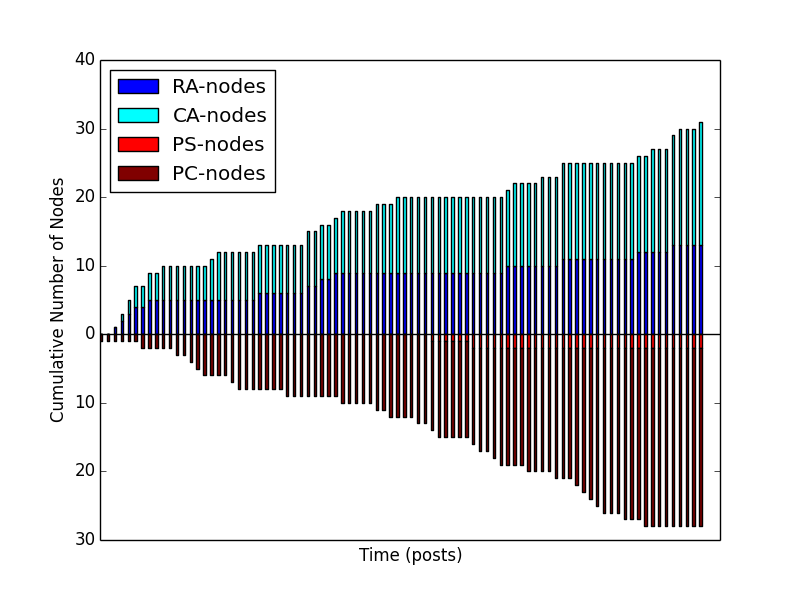
\includegraphics[scale=\scaleResults]{./figures/rhetoric_over_time/twitter.png}
\caption{Cumulative use of logical and rhetoric tactics over time on Twitter}
\label{figure:rhetorictime:Twitter}
\end{figure}

\begin{figure}
\centering
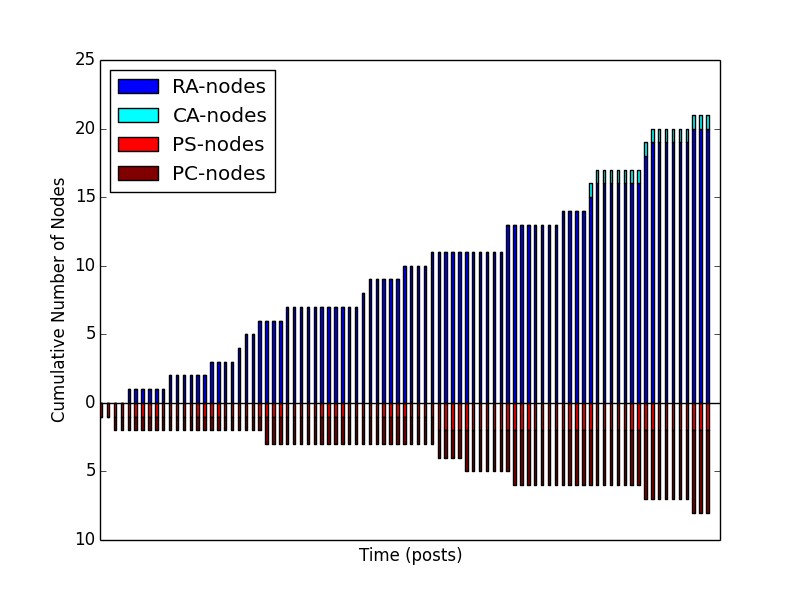
\includegraphics[scale=\scaleResults]{./figures/rhetoric_over_time/facebook.png}
\caption{Cumulative use of logical and rhetoric tactics over time on Facebook}
\label{figure:rhetorictime:Facebook}
\end{figure}

\begin{figure}
\centering
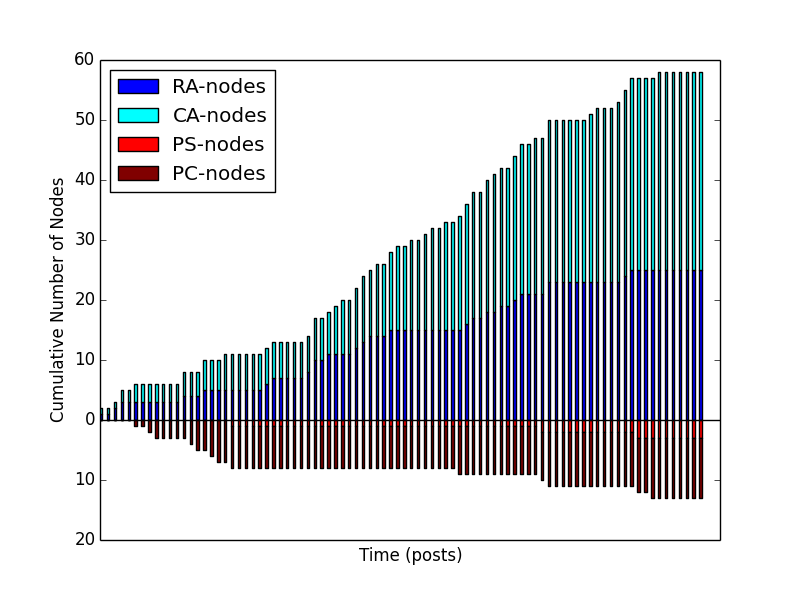
\includegraphics[scale=\scaleResults]{./figures/rhetoric_over_time/reddit.png}
\caption{Cumulative use of logical and rhetoric tactics over time on Reddit}
\label{figure:rhetorictime:reddit}
\end{figure}


\subsubsection{Argumentation Tactics per User}
In addition, proportion of logical versus rhetorical contributions made by each user is examined. These graphs show the contributions made by each user (ordered by total contributions overall). Once more, it must bed stressed that values below the x-axis should not considered anti-social solely due to their rhetorical nature.

Figures \ref{figure:rhetoricuser:Twitter} and \ref{figure:rhetoricuser:reddit} show that users in the Twitter and Reddit samples made more individual contributions to the argumentation structure than those in the Facebook sample, shown in Figure \ref{figure:rhetoricuser:Facebook}. This, along with the data in Table \ref{table:samples}, also supports the suggestion that there is more engagement in these communities than in the Facebook sample.

All samples also display a tendency for rhetorical contributions to be distributed across the scale, with (weak) grouping towards either end. 
This implies that the users most likely to employ rhetorical techniques are those that contribute the most posts to the discussion overall, and those that make no logical contributions at all.

\begin{figure}
\centering
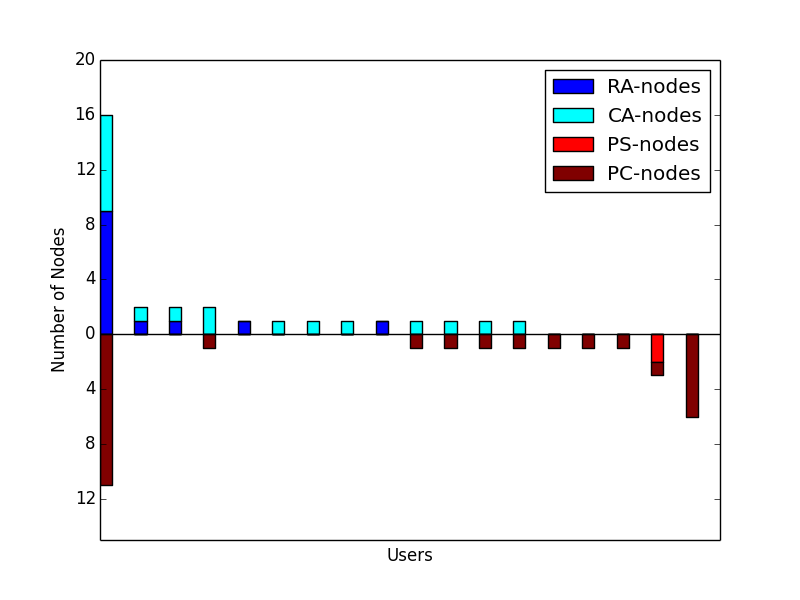
\includegraphics[scale=\scaleResults]{./figures/rhetoric_per_user/twitter.png}
\caption{Logical and rhetorical contributions per sampled user on Twitter}
\label{figure:rhetoricuser:Twitter}
\end{figure}

\begin{figure}
\centering
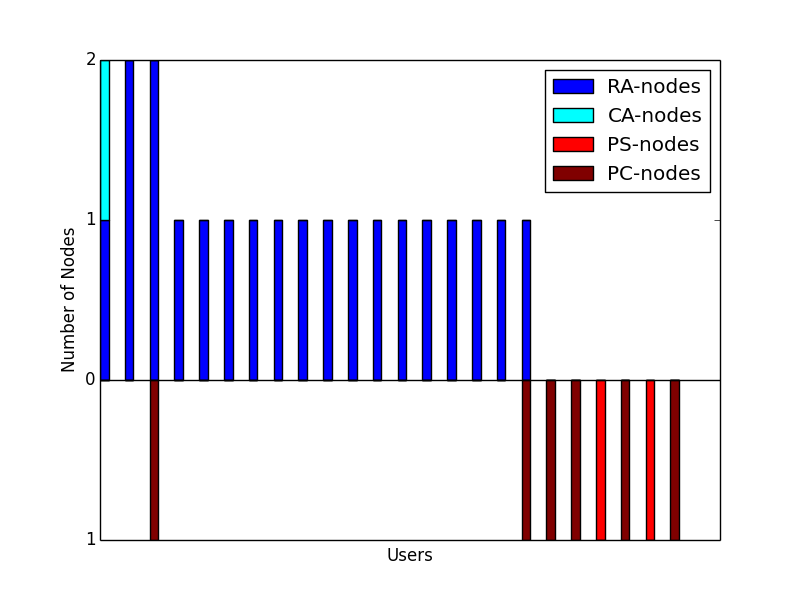
\includegraphics[scale=\scaleResults]{./figures/rhetoric_per_user/facebook.png}
\caption{Logical and rhetorical contributions per sampled user on Facebook}
\label{figure:rhetoricuser:Facebook}
\end{figure}

\begin{figure}
\centering
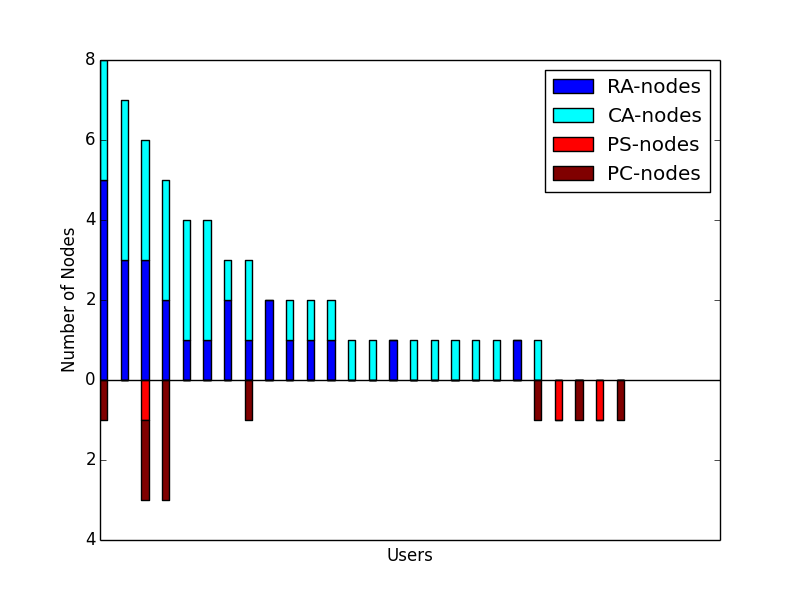
\includegraphics[scale=\scaleResults]{./figures/rhetoric_per_user/reddit.png}
\caption{Logical and rhetorical contributions per sampled user on Reddit}
\label{figure:rhetoricuser:reddit}
\end{figure}

\subsubsection{Correlation Between Argumentation Structure and Post Features}
Correlations were drawn between the structure of the annotated argument graph, including elements such as the number of logical or rhetorical supports or conflicts and replies to and from each post, and features of the post content and structure, such as post length, number of expletives, percentage of spelling errors and again, replies to and from the post. Replies in particular were viewed from both sides: that is, to analyse whether certain types of posts were more likely to be made in reply, or whether posts that were made in reply tended to contribute similar argumentation structures.

Due to the largely discrete (and often binary) nature of the features and values studied (the majority of posts, for example, are likely to contain either zero or one logical or rhetorical conflict) the correlations are relatively weak, as show in Figure \ref{figure:correlations:reddit}. However, some notable correlations are presented in Table \ref{table:correlations}. These show potential early indicators of the structure and value of an argument. For example, as might be expected, longer posts are more likely to have greater contributions to the discussion. Posts that use a large number of expletives are likewise more likely to contain a rhetorical attack. When examining all three case studies together, posts made in reply correlated with posts that were replied to, implying that when one or more users engage in a discussion, they are more likely to be engaged with in return.


\begin{figure}
\centering
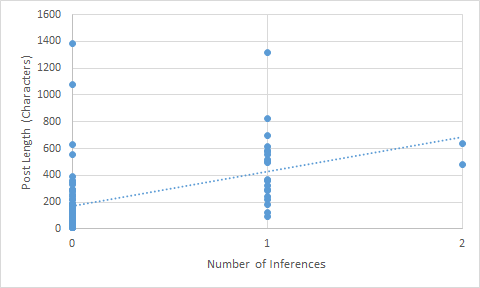
\includegraphics[scale=0.5]{./figures/correlations/reddit.png}
\caption{Post length correlated against number of logical inferences, on Reddit}
\label{figure:correlations:reddit}
\end{figure}



\begin{sidewaystable}
\centering
\caption{Notable correlations between structural argumentation annotations and post features}
\label{table:correlations}
\begin{tabular}{| l | l | l | c | c |}
\hline
\textbf{Case Study} & \textbf{Argumentation Structure} & \textbf{Post Feature} & \textbf{Pearson's Correlation (3 d.p.)} & \textbf{p-value (3 d.p.)}\\
\hline
Twitter & Personal attacks & Number of replies to this post & 0.325 & 0.002\\
\hline
Twitter & Personal attacks & Percentage of spelling errors & 0.301 & 0.004\\
\hline
Twitter & Personal attacks & Expletives & 0.462 & 0.000\\
\hline
Facebook & Original premises & Reputation (``Likes'') & 0.332 & 0.001\\
\hline
Facebook & Original conclusions & Reputation (``Likes'') & 0.329 & 0.002\\
\hline
Facebook & Logical inferences & Reputation (``Likes'') & 0.343 & 0.001\\
\hline
Facebook & Logical conflicts & Emoticons & 0.500 & 0.000\\
\hline
Facebook & Logical conflicts & Expletives & 0.397 & 0.000\\
\hline
Reddit & Original premises & Post length & 0.335 & 0.001\\
\hline
Reddit & Original conclusions & Post length & 0.333 & 0.001\\
\hline
Reddit & Logical inferences & Post length & 0.476 & 0.000\\
\hline
Reddit & Logical conflicts & Number of posts replied to & 0.435 & 0.000\\
\hline
Overall & Number of replies to this post & Number of posts replied to & 0.417 & 0.000\\
\hline
\end{tabular}
\end{sidewaystable}
